\section{Trasformata zeta}
La trasformata zeta aiuta l'analisi di stabilità e causalità delle frequenze dei sistemi lineari a tempo invariante con i relativi filtri, essendo più ampia rispetto alla trasformata di Fourier. La trasformata discreta non è sufficiente in alcune situazioni perché:
\begin{enumerate}
	\item Non sempre esiste;
	\item Descrive solo comportamenti di sistemi LTI scarichi;
	\item Presume condizioni iniziali nulle.
\end{enumerate}

La trasformata zeta è la parte discreta (digitale) della trasformata di Laplace, ed è rappresentata da una sommatoria con l'estensione delle frequenze nel mondo complesso, esprimibile in coordinate polari con un termine $\rho$ qualsiasi che determina la distanza dall'origine. L'operatore è lineare.

\begin{wrapfigure}{R}{0.4\textwidth}
	\vspace{-15pt}
	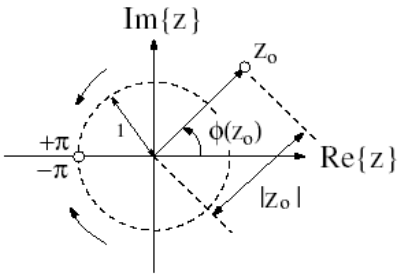
\includegraphics[width=0.4\textwidth]{Lezioni/Immagini/zeta}
	\vspace{-40pt}
\end{wrapfigure}

Data una frequenza bilatera $x(n)$ con $-\infty < n < \infty$ si definisce trasformata zeta:
$$X(z) = Z[x(n)] = \sum_{-\infty}^{\infty} x(n)z^{-n}$$
Esiste una corrispondenza biunivoca tra $x(z)$ e $x(n)$ e i loro domini solo se viene definita la regione di convergenza uniforme ROC, cioè i valori della variabile complessa $z$ tale che $x(z)$ è finita.

Nella regione di convergenza, $X(z)$ è una funzione analitica, cioè continua e indefinitamente derivabile con derivate continue in $z$.

La $z$ è una pulsazione complessa con dominio $\mathcal{C}$, rappresentabile in termini di modulo e fase come $z = \rho e^{j2\pi f} = \rho e^{j\omega}$. Si può ridurre a trasformata di Fourier discreta togliendo il coefficiente complesso e applicando la formula a una nuova sequenza. 

Deve valere la condizione di sommabilità in modulo, quindi la convergenza varia con la distanza e il piano si può dividere in circonferenze concentriche con comportamento diverso. 

La regione ROC dipende solo dal modulo $\rho$ delle pulsazioni complesse $z$, e non dalla loro fase: questo comporta le circonferenze come luoghi dei punti $z$ a modulo costante.
$$ \sum_{-\infty}^{\infty}\abs{x(n)\rho^{-n}} < \infty \implies  \sum_{-\infty}^{\infty}\abs{x(n)}\rho^{-n} < \infty$$
In particolare, è importante trovare i valori di $\rho$ che indicano la convergenza, e si ha che i valori sulla circonferenza di raggio unitario $\rho = 1$ sono i valori della trasformata di Fourier di frequenza 0. Quando c'è un ritardo, la regione sarà individuata con $[z \neq 0]$.

\begin{figure}[h]
	\centering
	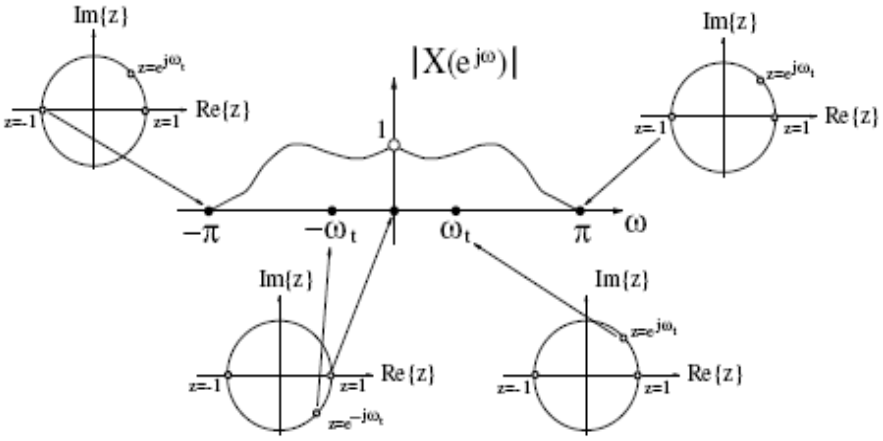
\includegraphics[scale=0.35]{Lezioni/Immagini/zdft}
\end{figure}

\subsection{Trasformate e ROC}
La trasformata zeta definisce una relazione biunivoca tra la sequenza $x(n)$ e una funzione della variabile complessa $z$. La biunivocità è garantita solo se si specifica la ROC di $X(z)$ e l'espressione analitica della trasformata.

Esistono relazioni specifiche tra la tipologia di una generica sequenza $x(n)$ e la ROC della relativa trasformata $z$:
\begin{itemize}
	\item Le sequenze $x(n)$ bilatere hanno supporto che si estende sia su istanti di tempo discreto negativi che positivi;
	\item Le sequenze causali possiedono coefficienti identicamente nulli per istanti di tempo negativi, origine esclusa;
	\item Le sequenze causali possiedono coefficienti identicamente nulli per istanti di tempo positivi.
\end{itemize}

\subsubsection{Impulso $\delta$}
$$X(z) = \sum_{-\infty}^{\infty} \delta(n) z^{-n} = 1$$
Se l'impulso $x(n) = \delta(n)$ è una costante nel dominio trasformato, applicando la funzione zeta si ha un risultato simile: tutti i valori assumono 0 tranne quello per cui $n = 0$, quindi l'esponenziale diventa 1 così come tutta la trasformata. 

La regione di convergenza è costante e limitata a 1, e rappresenta tutto il piano complesso per cui la serie geometrica converge.
$$x(n) = 2\delta(n+1) + \delta(n) + 4\delta(n-2) = 2\sum_{-\infty}^{\infty}2\delta(n+1)z^{-n} + \sum_{-\infty}^{\infty}2\delta(n)z^{-n} + 4\sum_{-\infty}^{\infty}2\delta(n-2)z^{-n}$$
$$\implies 2z + 1 + 4z^{-2}$$
Il risultato è ottenuto scomponendo le sommatorie e trovando i valori per cui il numero all'interno delle parentesi si annulla. Bisogna sempre tenere conto del segno negativo dell'esponente.

\subsubsection{Gradino}
$$X(z) = \sum_{-\infty}^{\infty}u(n)z^{-n} = \sum_{0}^{\infty}z^{-n} = \sum_{0}^{\infty}\big(z^{-1}\big)^n = \frac{1}{1 - z^{-1}}$$
In una sequenza a gradino, la ROC corrisponde all'esterno della circonferenza di raggio unitario, cioè $\big[\abs{z^{-1}} < 1 \geq \abs{z} > 1\big]$. La stessa formula vale per il gradino anticausale, e la corrispondenza biunivoca si ritrova perché la ROC cambia in $\abs{z} < 1$.

% slide 11
\subsubsection{Finestra}
Finestra: caratterizzata da un esponenziale $\alpha^n$, di cui viene considerata solo una parte. La $x(z)$ è un rapporto tra polinomi, e la $h(z)$ sarà simile. La trasformata converge per $z \neq 0$.

Essendoci polinomi, sia il numeratore che il denominatore potrebbero annullarsi: nel primo caso si chiamano zeri, altrimenti poli. Per individuare i valori si può raccogliere i fattori arrivando all'ordine 1 nel denominatore.

In questo caso i campioni infiniti vengono rappresentati come rapporto finito di polinomi infiniti.

C'è una parte in comune $z = \alpha$ che annulla sia denominatore che numeratore, quindi gli zeri corrispondenti si semplificano e la sequenza resta finita. Ci sono $N - 1$ poli per $z = 0$.

Gli zeri si posizionano in modo uniforme a intervalli distanti uguali, nelle pulsazioni complesse. 

Serie geometrica:

In altre parole, sequenze causali = esterno della circonferenza, sequenze anticausali = interno.

L'importante è ragionare sui poli, che determinano la convergenza in base alla causalità. Il numero di poli e zeri corrisponde all'ordine, che può essere diverso tra numeratore e denominatore.

La frequenza è legata alla posizione angolare, quindi essendo i poli in zero la loro influenza si riflette su tutte le frequenze o nessuna: il contributo è nullo.

Studiando i poli si analizza la regione in cui la funzione viene amplificata e cresce in valore, gli zeri dove diminuisce. Insieme quindi danno l'andamento delle frequenze.

I coefficienti nell'equazione alle differenze corrispondono ai coefficienti nella trasformata, considerando il cambiamento di segno. Al numeratore c'è la parte non ricorsiva, e al denominatore quella ricorsiva. Se non c'è il denominatore, la sequenza è FIR.

Il sistema è stabile se la trasformata di Fourier è interna alla regione di convergenza. 



